\documentclass[12pt]{article}
\usepackage[utf8]{inputenc}
\usepackage[T1]{fontenc}	
\usepackage{array,latexsym}
\usepackage{amsmath,amsfonts,amssymb,amsthm,mathabx,amstext}
\usepackage{dsfont}	% Conjuntos: $\mathds{N, Z, Q, R, C}$
\usepackage{graphicx}

\begin{document}
	
	\pagestyle{empty}
	
	\begin{center}
		Universidade Federal da Paraíba\\
		Bacharelado em Estatística\\
		Probabilidade II - Exercícios de teoria de conjuntos\\
		Paulo Ricardo Seganfredo Campana\\
	\end{center}

	1. Quais dos conjuntos abaixo são vazios?\\

	\noindent Apenas os conjuntos\\
	\( B=\lbrace x:x>\frac{9}{4}\:\text{e}\:x<\frac{6}{5}\rbrace \) e \( D=\lbrace x:x \:\text{divisível por zero} \rbrace \)\\
	
	2. Construa o conjunto das partes do conjunto $A=\lbrace a, b, c, d\rbrace$
	\vspace{12pt}
  	
  	\noindent\( A = \lbrace \varnothing, \lbrace a \rbrace, \lbrace b \rbrace, \lbrace c \rbrace, \lbrace d \rbrace, \lbrace a, b \rbrace, \lbrace a, c \rbrace, \lbrace a, d \rbrace, \lbrace b, c \rbrace, \lbrace b, d \rbrace, \lbrace c, d \rbrace,\\ \lbrace a, b, c \rbrace, \lbrace a, b, d \rbrace, \lbrace a, c, d \rbrace, \lbrace b, c, d \rbrace, A \rbrace \)\\
  	
  	3. Diga se é verdadeira (V) ou falsa (F) cada uma das sentenças abaixo. Se a sentença for falsa deverá ser justificada.
  	\vspace{12pt}
  	
  	\noindent a) V\\
  	b) F, o elemento a pertence ao conjunto $\lbrace a, b\rbrace$, porém o conjunto $\lbrace a \rbrace$ não pertence\\
  	c) V\\
  	d) F, zero não pertence ao conjunto vazio pois o mesmo não possui elementos\\
  	e) F, pois apenas o elemento $ \varnothing\:\text{pertence ao conjunto}\:\varnothing $ \\
  	f) V\\
  	g) V\\
  	h) V\\
  	i) V\\
  	j) F, os elementos do conjunto $\lbrace a, b \rbrace$ pertencem a $\lbrace \lbrace a, b, c, d \rbrace \rbrace$ porém o conjunto $\lbrace a, b \rbrace$ não pertence\\
  	
  	4. Dados os conjuntos $A = \{a, b, c, d\}$, $B = \{b, c, d, e\}$ e $C = \{c, e, f\}$, determine $A \cap B$, $A \cap C$, $B \cap C$
  	e $A \cap B \cap C$, $A \cup B$, $A \cup C$, $B \cup C$ e $A \cup B \cup C$. Verifique também se cada reunião é disjunta.\\
  	\vspace{12pt}
  	
  	\noindent $A \cap B = \{b,c,d\}$\\
  	$A \cap C = \{c\}$\\
  	$B \cap C = \{c, e\}$\\
  	$A \cap B \cap C = \{c\}$\\
  	$A \cup B = \{a,b,c,d,e\}$\\
  	$A \cup C = \{a,b,c,d,e,f\}$\\
  	$B \cup C = \{b,c,d,e,f\}$\\
  	$A \cup B \cup C = \{a,b,c,d,e,f\}$\\\\
  	Não, todas possuem o elemento $c$.\\
  	 
  	5.  Prove que $A \subset (A \cup B)$, $(A \cap B) \subset A$ e que $(A-B) \subset A$, $\forall A$\\
  	\vspace{12pt}
  	
  	\noindent a) $A \subset (A \cup B)$, pelas definições de subconjunto e união:\\
  	$\forall x, (x \in A \Rightarrow x \in (A \cup B)) $\\
  	$\forall x, (x \in A \Rightarrow x \in A\:\text{ou}\: x \in B) $\\
  	$\forall x, (x \in A \Rightarrow x \in A)$\\\\
  	
  	\noindent b) $(A \cap B) \subset A$ pelas definições de subconjunto e interseção:\\
  	$\forall x, (x \in (A \cap B) \Rightarrow x \in A)$\\
  	$\forall x, (x \in A\:\text{e}\:x \in B \Rightarrow x \in A)$\\
  	$\forall x, (x \in A \Rightarrow x \in A)$\\\\
  	
  	\noindent c) $(A-B) \subset A$, $\forall A$, pelas definições de subconjunto e diferença:\\
  	$\forall x, (x \in (A-B) \Rightarrow x \in A)$\\
  	$\forall x, (x \in (A \cap B^{c}) \Rightarrow x \in A)$\\
  	$\forall x, (x \in A\:\text{e}\: x \in B^{c}) \Rightarrow x \in A)$\\
  	$\forall x, (x \in A \Rightarrow x \in A)$\\
  	
  	6. Admitindo que A, B e C são conjuntos quaisquer, classifique em verdadeiro (V) ou falso (F) as seguintes sentenças:
  	\vspace{12pt}
  	
  	\noindent a) V \quad b) F \quad c) F \quad d) V \quad e) V \quad f) V\\
  	g) V \quad h) F \quad i) F \quad j) V \quad k) V \quad l) V\\
  	
  	7. Indique no diagrama abaixo, um de cada vez, os seguintes conjuntos:\\\\\\\\
  	\vspace{12pt}
  	
  	\begin{figure}[h!]
  		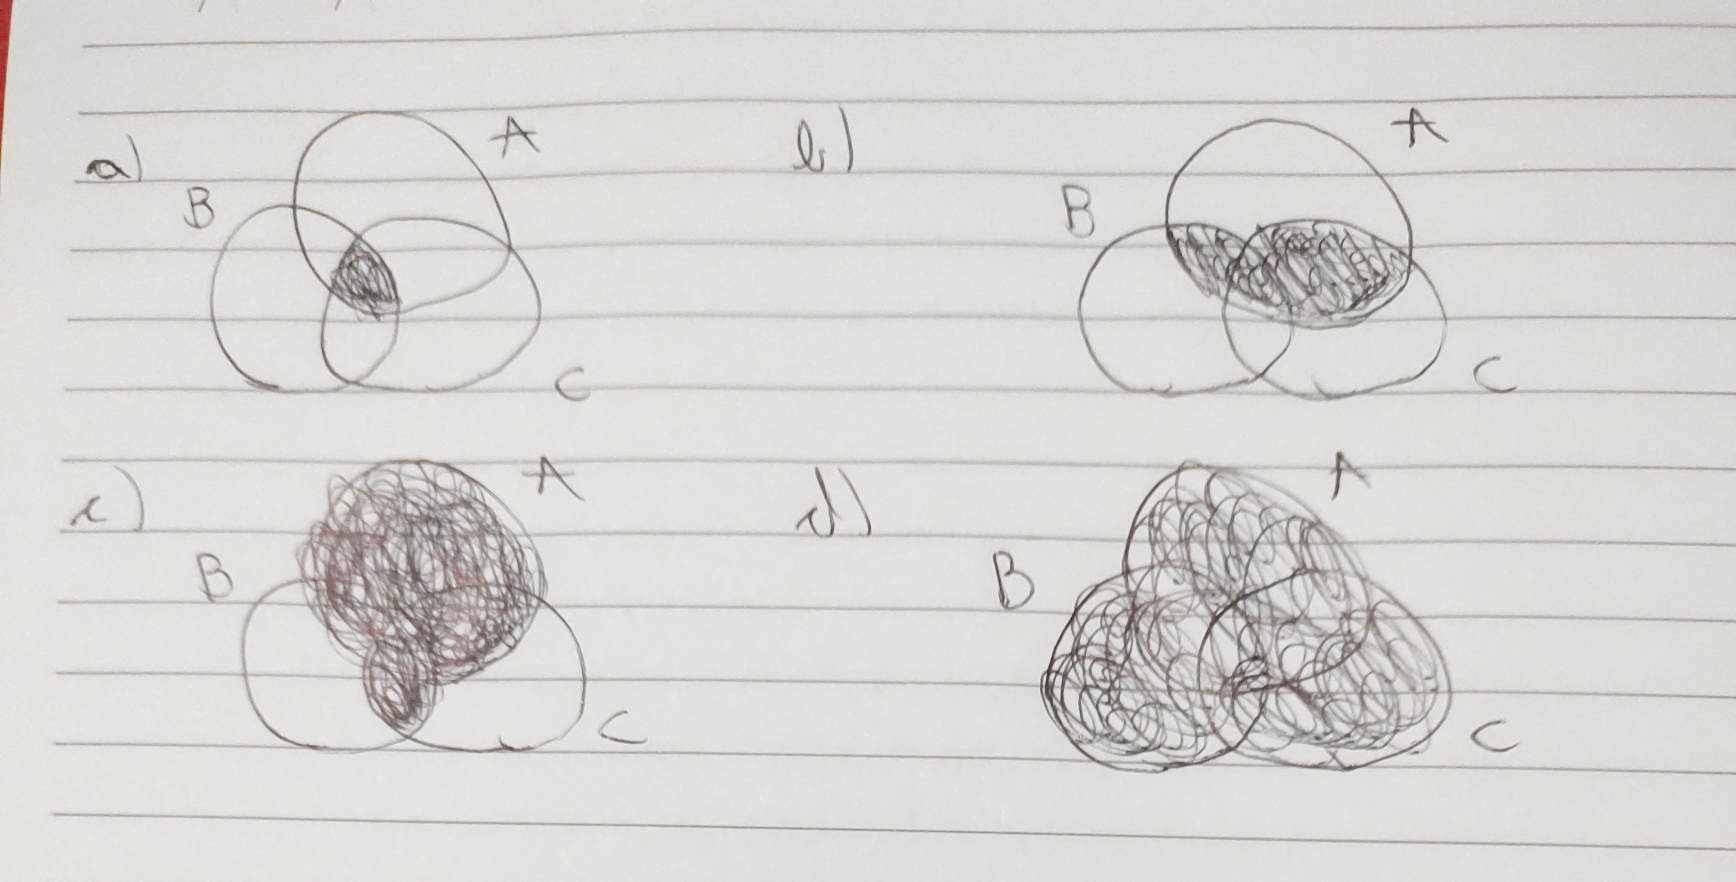
\includegraphics[scale=0.2]{q7}
  	\end{figure}
  
  	8. Sejam os conjuntos $A = \{a, b, c, d\}$, $B = \{c, d, e, f, g\}$ e $C = \{b, d, e, g\}$. determine:
  	\vspace{12pt}
  	
  	\noindent a) $A-B = \{c,d\}$\\
  	b) $B-A = \{e,f,g\}$\\
  	c) $C-B = \{b\}$\\
  	d) $(A \cup C)-B = \{a,b\}$\\
  	e) $A-(B \cap C) = \{a,b,c\}$\\
  	f) $(A \cup B)-(A \cap C) = \{a,c,e,f,g\}$\\
  	
  	9. Faça um diagrama para indicar cada um dos conjuntos abaixo:\\\\\\\\\\\\\\\\\\\\\\\\\\\\
  	\vspace{12pt}
  	
  	\begin{figure}[h!]
  		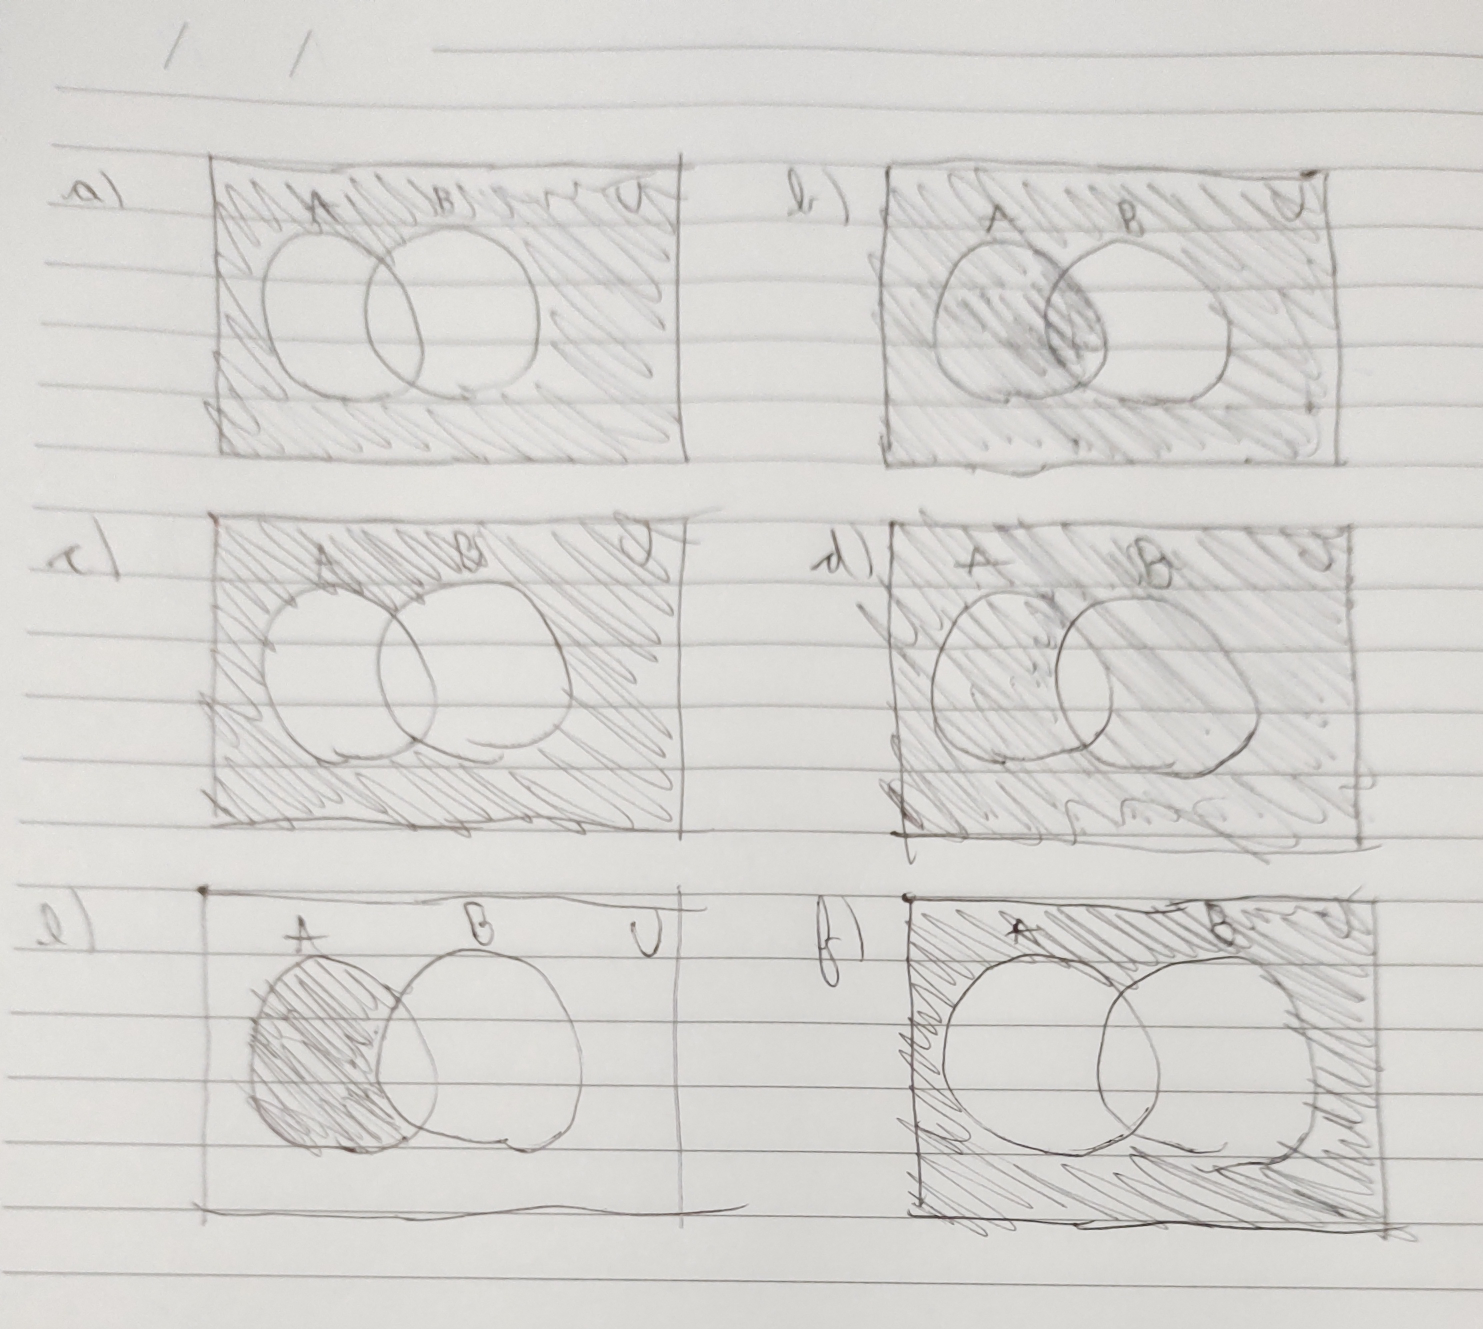
\includegraphics[scale=0.2]{q9}
  	\end{figure}
  
  	10. Dados dois conjuntos $A$ e $B$, chama-se a diferença simétrica de $A$ com $B$ o conjunto tal que: $A\Delta B = (A-B)\cup (B-A)$. Prove que:\\
  	\vspace{12pt}	
  	
  	\noindent a) $A\Delta \varnothing = A$\\
  	$(A-\varnothing)\cup(\varnothing-A) = A$\\
  	$(A\cap \varnothing^{c})\cup(\varnothing \cap A^{c}) = A$\\
  	$(A\cap U)\cup(\varnothing) = A$\\
  	$A = A$\\\\
  	
  	\noindent b) $A\Delta A = \varnothing$\\
  	$(A-A)\cup(A-A) = \varnothing$\\
  	$\varnothing \cup \varnothing = \varnothing$\\
  	$\varnothing = \varnothing$\\\\
  	
  	\noindent c) $A\Delta B = B\Delta A$ para $A$ e $B$ quaisquer.\\
  	$(A-B)\cup(B-A) = B\Delta A$\\
  	$(B-A)\cup(A-B) = B\Delta A$\\
  	$B\Delta A = B\Delta A$\\
  	
  	11. Sejam A, B e C três conjuntos quaisquer. Demonstre que:
  	\vspace{12pt}
  	
  	\noindent a) $(A-C)\cup(B-C) = (A\cup B)-C$\\
  	$(A\cap C^{c})\cup(B\cap C^{c}) = (A\cup B)\cap C^{c}$\\
  	$C^{c}\cap(A\cup B) = (A\cup B)\cap C^{c}$\\
  	$C^{c}\cap(A\cup B) = C^{c}\cap(A\cup B)$\\\\
  	
  	\noindent b) $(A-C)\cap(B-C) = (A\cap B)-C$\\
  	$ (A \cap C^{c}) \cap (B \cap C^{c}) = (A \cap B) \cap C^{c} $\\
  	$ A \cap B \cap C^{c} = (A \cap B) \cap C^{c} $\\
  	$ (A \cap B) \cap C^{c} = (A \cap B) \cap C^{c} $\\
  	
  	12. Sejam $A$ e $B$ conjuntos quaisquer. Demonstre que $A$ e $B-A$ são disjuntos, e que $A\cup B = A\cup (B-A)$. Isso mostra como representar $A\cup B$ como uma união disjunta.
    \vspace{12pt}
  	
  	\noindent  Assuma que $A$ e $B$ não são disjuntos, isso significa que:\\
  	$ A \cap (B-A) \neq \varnothing $\\
  	$ A \cap (B \cap A^{c}) \neq \varnothing $\\
  	$ (A \cap A^{c}) \cap B \neq \varnothing $\\
  	$ \varnothing \cap B \neq \varnothing $\\
  	$ \varnothing \neq \varnothing $ \\
  	Há uma contradição, que significa que $A$ e $B$ são de fato disjuntos.\\\\
  	
  	\noindent $A\cup B = A\cup(B-A)$\\
  	$A\cup B = A\cup(B\cap A^{c})$\\
  	$A\cup B = (A\cup B)\cap(A\cup A^{c})$\\
  	$A\cup B = (A\cup B)\cap U$\\
  	$A\cup B = A\cup B$\\
  	
\end{document}